\documentclass{article}
\usepackage{graphicx}
\usepackage{amssymb}
\usepackage{amsmath}
\usepackage{tikz}
\usepackage{url}
\usepackage{color}
% \usepackage{savetrees}
\usepackage{listings}
% \usetikzlibrary{shapes}

% pseudocode notations
\newcommand{\xif}{{\bf{\em{if~}}}}
\newcommand{\xthen}{{\bf{\em{then~}}}}
\newcommand{\xelse}{{\bf{\em{else~}}}}
\newcommand{\xelseif}{{\bf{\em{elif~}}}}
\newcommand{\xfi}{{\bf{\em{fi~}}}}
\newcommand{\xcase}{{\bf{\em{case~}}}}
\newcommand{\xendcase}{{\bf{\em{endcase~}}}}
\newcommand{\xfor}{{\bf{\em{for~}}}}
\newcommand{\xto}{{\bf{\em{to~}}}}
\newcommand{\xby}{{\bf{\em{by~}}}}
\newcommand{\xdownto}{{\bf{\em{downto~}}}}
\newcommand{\xdo}{{\bf{\em{do~}}}}
\newcommand{\xrof}{{\bf{\em{rof~}}}}
\newcommand{\xwhile}{{\bf{\em{while~}}}}
\newcommand{\xendwhile}{{\bf{\em{endwhile~}}}}
\newcommand{\xand}{{\bf{\em{and~}}}}
\newcommand{\xor}{{\bf{\em{or~}}}}
\newcommand{\xerror}{{\bf{\em{error~}}}}
\newcommand{\xreturn}{{\bf{\em{return~}}}}
\newcommand{\xparallel}{{\bf{\em{parallel~}}}}
\newcommand{\T}{\hspace{0.5cm}}
\newcommand{\m}{\mathcal}

\def\func#1{\textrm{\bf{\sc{#1}}}}
\def\funcbf#1{\textrm{\textbf{\textsc{#1}}}}


\linespread{1.5}
\setlength{\parindent}{0pt}
\setlength{\parskip}{1.9ex plus 0.5ex minus 0.2ex}

% \linespread{1.4}

\title{CSE613\\Parallel Programming -- Homework-2}

\author{Dhruv Matani (108267786) \& Gaurav Menghani (108266803)}

\renewcommand{\thesubsection}{\thesection\ (\alph{subsection})}

\begin{document}
\maketitle

\clearpage

\tableofcontents

\clearpage

\section{Parallel BFS with Split Queues}

Compiling all the programs:
\begin{verbatim}
$ make
\end{verbatim}

The generated executables are as follows:

\begin{enumerate}
\item \textbf{serial}: The executable for running the serial code.
\item \textbf{parallel}: The executable for the parallel code without work stealing, but with the O(1) time queue splice optimization.
\item \textbf{parallel\_d}: The same as \textit{parallel} except that part-(d) is also implemented.
\item \textbf{parallel\_h}: The same as \textit{parallel} except that part-(h) is also implemented.
\end{enumerate}

To enable the modifications of part (f), you need to run:
\begin{verbatim}
$ make FLAGS="-DPARTF" CILKFLAGS="-lmiser"
\end{verbatim}


\subsection{Serial BFS}

Please check archive for the code

Running the code:
\begin{verbatim}
$ ./serial < input_file_path
\end{verbatim}

\subsection{Parallel BFS}

Running the code:
\begin{verbatim}
$ ./parallel < input_file_path
\end{verbatim}

\subsection{Analysis of race conditions}

\texttt{PARALLEL-BFS} may give rise to race conditions because a
vertex \textit{v} might be added to the queue multiple times by
different threads and that vertex might then be expanded multiple
times by different threads at the same time. These threads might
simultaneously update the distance value for vertex \textit{v}.

The output will still be correct because this race is benign. Despite
the fact that multiple threads will add a vertex \textit{v} to the
queue, they will all set the distance of vertex \textit{v} from the
source vertex \textit{s} as the same value, so the output will remain
correct.

\subsection{Single expansion of a vertex}

In any given iteration of the \textit{while} loop, more than one
process works to expand a vertex \textit{u}. It is possible that
vertices \textit{u} and \textit{u'} both point to vertex
\textit{v}. In this case, it is possible that 2 processors are
processing vertices \textit{u} and \textit{u'}, and they both happen
to check the value of \textit{d[v]} at the same time and find it to be
$\infty$. They will both set it to the same value, and add vertex
\textit{v} to each of their queues. Hence, the same vertex \textit{v}
might appear more than once in $Q_{in}$.

However, a vertex \textit{v} will \textit{not} appear more than once
in any queue \textit{q} in $Q_{in}$ since the code that populates a
queue \textit{q} in $Q_{out}$ executes serially and will necessarily
check $d[v]$ before adding vertex \textit{v} to its queue.

We re-write \texttt{PARALLEL-BFS-THREAD} as follows to include the
parent node \textit{p} of a vertex \textit{v} that caused the vertex
\textit{v} to be explored. We also maintain a separate \textit{parent}
array that stores the parent node due to which a vertex \textit{v} was
added to some queue for further expansion. If the value of parent node
when fetched from the queue matches that of the parent node for vertex
\textit{v} in the \textit{parent} array, then we process the vertex
\textit{v}, otherwise we do \textit{not} process it.

\vspace{0.2cm}
\noindent
\begin{enumerate}

\item \func{PARALLEL-BFS-THREAD\ ($G, Q^i, Q^o, d$)}

\item \xwhile ($S = Q^i.nextSegment()$) $\neq \emptyset$ \xdo

\item \T \xwhile ($S \neq \emptyset$) \xdo

\item \T \T $(p, u) \leftarrow S.extract()$

\item \T \T \xif $parent[u] = p$ \xthen

\item \T \T \T \xfor each $v \in \tau(u)$ \xdo

\item \T \T \T \T \xif $d[v] = +\infty$ \xthen

\item \T \T \T \T \T $d[v] \leftarrow d[u] + 1$

\item \T \T \T \T \T $Q^o.enque((u, v))$

\item \T \T \T \T \T $parent[v] \leftarrow u$

\end{enumerate}

\subsection{Efficient implementation of \textit{Q.nextSegment}}

To implement the function \textit{Q.nextSegment} efficiently, we don't
actually copy the values in the queue. Instead we maintain pointers
into the queue that contains the range of elements that need to be
processed. So the set $S$ that is returned by \textit{Q.nextSegment}
is not a set containing the actual elements, but just a pair of
pointers to the elements in some queue $q$ of $Q_{in}$.

If we set $n_{seg}$ to $p$, the number of processing elements, then
$s_{seg} = \frac{Q_{in}}{n_{seg}} = \frac{Q_{in}}{p}$.

Since the amount of time spent in call of \textit{Q.nextSegment} is
amortized $O(1)$, the total number of non-full sets returned by
\textit{Q.nextSegment} will be at most $p$. Hence, the total time
spent in \textit{Q.nextSegment} in each iteration of the
\textit{while} loop will be $O(p)$.

\subsection{Optimizing space used by $Q^{in}$ and $Q^{out}$}

To compile, type:
\begin{verbatim}
$ make FLAGS="-DPARTF" CILKFLAGS="-lmiser"
\end{verbatim}

\subsection{Work \& Span of \texttt{PARALLEL-BFS}}

The total work done ($T_1$) by all implementations of
\texttt{PARALLEL-BFS} is $O(V + E)$.

The span ($T_\infty$) for either implementation in the worst case
would be $O(V)$ if the graph is a linked list, since each vertex
\textit{v} would be processed only after its parent vertex \textit{u}
is processed.

However, for a graph with a diameter $D$, the span ($T_\infty$) would
be $O(D)$.

\subsection{\texttt{PARALLEL-BFS} with work-stealing}

You can run this program by typing:
\begin{verbatim}
$ ./parallel_h < input_file_path
\end{verbatim}

\subsection{Tabular comparison}

\begin{center}
  \begin{tabular}{| l | r | r | r | r |}
    \hline
    Input/Algorithm & (a) & (b) & (d) & (h) \\ \hline
    \texttt{test-01-in.txt} & 41sec & 21sec (1.95 x) & 26sec (1.58x) & 28sec (1.46x) \\ \hline
    \texttt{test-02-in.txt} & 1min 4sec & 17sec (3.76 x) & 23sec (2.84x) & 18sec (3.55x) \\ \hline
    \texttt{test-03-in.txt} & 23min 22sec & 5min 20s (4.38 x) & 4min 40sec (5.00x) & 4min 39sec (5.02x) \\ \hline
    \texttt{test-04-in.txt} & 16min 23sec & 2min 28sec (6.64x) & 2min 47sec (5.72x) & 2min 45sec (5.92x) \\
    \hline
  \end{tabular}
\end{center}

\subsection{\textit{Cilkview} scalability plot}
\begin{figure}[h!]
  \begin{center}
    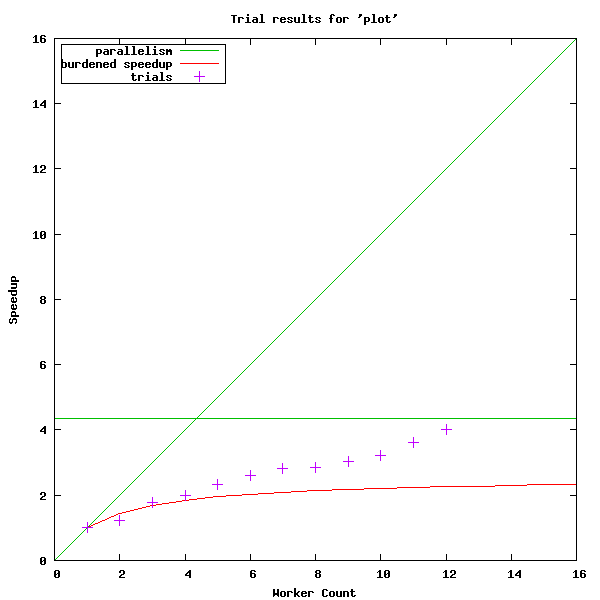
\includegraphics[width=4in]{plots/plot_part_b.png}
    \caption{Cilkview plot for part(b)}
    \label{fig:cilkview_b}
  \end{center}
\end {figure}

\begin{figure}[h!]
  \begin{center}
    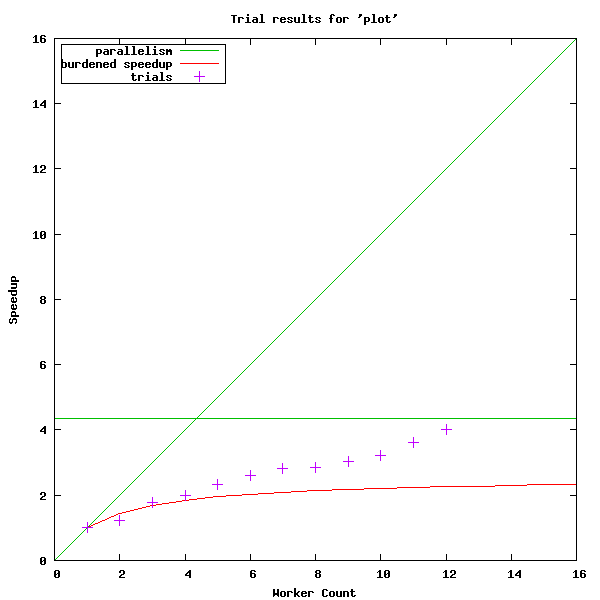
\includegraphics[width=4in]{plots/plot_part_h.png}
    \caption{Cilkview plot for part(h)}
    \label{fig:cilkview_h}
  \end{center}
\end {figure}

\end{document}
